\documentclass[12pt,letterpaper]{article}
\usepackage{graphicx,textcomp}
\usepackage{natbib}
\usepackage{setspace}
\usepackage{fullpage}
\usepackage{color}
\usepackage[reqno]{amsmath}
\usepackage{amsthm}
\usepackage{fancyvrb}
\usepackage{amssymb,enumerate}
\usepackage[all]{xy}
\usepackage{endnotes}
\usepackage{lscape}
\newtheorem{com}{Comment}
\usepackage{float}
\usepackage{hyperref}
\newtheorem{lem} {Lemma}
\newtheorem{prop}{Proposition}
\newtheorem{thm}{Theorem}
\newtheorem{defn}{Definition}
\newtheorem{cor}{Corollary}
\newtheorem{obs}{Observation}
\usepackage[compact]{titlesec}
\usepackage{dcolumn}
\usepackage{tikz}
\usetikzlibrary{arrows}
\usepackage{multirow}
\usepackage{subcaption}
\usepackage{xcolor}
\newcolumntype{.}{D{.}{.}{-1}}
\newcolumntype{d}[1]{D{.}{.}{#1}}
\definecolor{light-gray}{gray}{0.65}
\usepackage{url}
\usepackage{listings}
\usepackage{color}

\definecolor{codegreen}{rgb}{0,0.6,0}
\definecolor{codegray}{rgb}{0.5,0.5,0.5}
\definecolor{codepurple}{rgb}{0.58,0,0.82}
\definecolor{backcolour}{rgb}{0.95,0.95,0.92}

\lstdefinestyle{mystyle}{
	backgroundcolor=\color{backcolour},   
	commentstyle=\color{codegreen},
	keywordstyle=\color{magenta},
	numberstyle=\tiny\color{codegray},
	stringstyle=\color{codepurple},
	basicstyle=\footnotesize,
	breakatwhitespace=false,         
	breaklines=true,                 
	captionpos=b,                    
	keepspaces=true,                 
	numbers=left,                    
	numbersep=5pt,                  
	showspaces=false,                
	showstringspaces=false,
	showtabs=false,                  
	tabsize=2
}
\lstset{style=mystyle}
\newcommand{\Sref}[1]{Section~\ref{#1}}

\title{Assignment 1}
\date{Applied Stats/Quant Methods 1}
\author{Ella Karagulyan}

\begin{document}
	\maketitle
	
\section*{Question 1 }

\textit{A school counselor was curious about the average IQ of the students in her school and took a random sample of 25 students’ IQ scores.}\\
\vspace{.2cm}

\noindent First, we load the dataset.\\

\lstinputlisting[language=R, firstline=37, lastline=37]{PS01_answers_EK.R} 
\vspace{.2cm}

\noindent Next, we find the  90\% confidence interval for the mean student IQ in the school. 
\vspace{.2cm}

\lstinputlisting[language=R, firstline=39, lastline=39]{PS01_answers_EK.R} 
\vspace{.2cm}

\noindent The mean student IQ in the school is 98.44  with 90\% CI [93.96, 102.92]. 
Below are the  results of the One-sample t-test. \\

\begin{verbatim}
One Sample t-test

data:  y
t = 37.593, df = 24, p-value < 2.2e-16
alternative hypothesis: true mean is not equal to 0
90 percent confidence interval:
93.95993 102.92007
sample estimates:
mean of x 
98.44 
\end{verbatim}

\noindent \textit{Next, the school counselor was curious whether the mean student IQ in her school is higher than the mean IQ score (100) among all the schools in the country.}\\
\vspace{.2cm}

\noindent To test this we need to conduct a one-tailed t-test.  \\

\lstinputlisting[language=R, firstline=40, lastline=40]{PS01_answers_EK.R} 
\vspace{.2cm}

\noindent The One-sample t-test results provide no statistically significant evidence to conclude that the mean students' IQ of 98.4 (95\% CI[93.96, $\infty$]) is greater than 100, t(24)=-0.6, p=0.72.\\

\begin{verbatim}
One Sample t-test

data:  y
t = -0.59574, df = 24, p-value = 0.7215
alternative hypothesis: true mean is greater than 100
95 percent confidence interval:
93.95993      Inf
sample estimates:
mean of x 
98.44 
\end{verbatim}
\vspace{.2cm}

\noindent We also checked whether mean students' IQ is equal to the mean IQ score (100) among all the schools in the country. 
\vspace{.2cm}

\lstinputlisting[language=R, firstline=41, lastline=41]{PS01_answers_EK.R}  
\vspace{.2cm}

\noindent  The One-sample t-test results provide no statistically significant evidence to conclude that the mean students' IQ of 98.4 (95\% CI[93.03, 103.84]) isequal to 100, t(24)=-0.6, p=0.56.\\
Below are the results of the One-sample t-test.\\

\begin{verbatim}
	One Sample t-test

data:  y
t = -0.59574, df = 24, p-value = 0.5569
alternative hypothesis: true mean is not equal to 100
95 percent confidence interval:
93.03553 103.84447
sample estimates:
mean of x 
98.44 
\end{verbatim}
\vspace{.2cm}

\section*{Question 2}

\noindent \textit{Researchers are curious about what affects the amount of money communities spend on addressing homelessness. The following variables constitute our data set about social welfare expenditures in the USA.}\\

\begin{tabular}{r|l}
	\texttt{State} &\emph{50 states in US} \\
	\texttt{Y} & \emph{per capita expenditure on shelters/housing assistance in state}\\
	\texttt{X1} &\emph{per capita personal income in state} \\
	\texttt{X2} &  \emph{Number of residents per 100,000 that are "financially insecure" in state}\\
	\texttt{X3} &  \emph{Number of people per thousand residing in urban areas in state} \\
	\texttt{Region} &  \emph{1=Northeast, 2= North Central, 3= South, 4=West} \\
	
\end{tabular}
\vspace{.2cm}

\noindent First, we load the dataset, assign labels to variables and its categories for ease of use and explore the data. \\

\lstinputlisting[language=R, firstline=47, lastline=59]{PS01_answers_EK.R} 

\begin{verbatim}
Y	      									X1	      						X2														X3
Min.   : 42.00  	Min.   :1053  	Min.   :111.0  	Min.   :326.0  
1st Qu.: 67.25  	1st Qu.:1698  	1st Qu.:187.2  	1st Qu.:426.2  
Median : 79.00  	Median :1897  	Median :241.5  	Median :568.0  
Mean   : 79.54  	Mean   :1912  	Mean   :281.8  	Mean   :561.7  
3rd Qu.: 90.00  	3rd Qu.:2096  	3rd Qu.:391.8  	3rd Qu.:661.2  
Max.   :129.00  	Max.   :2817  	Max.   :531.0  	Max.   :899.0  

STATE														REGION		
Length:50         	Northeast    : 9  		
Class :character  	North Central:12  		
Mode  :character  	Southeast    :16  		
																			West         :13  		              
\end{verbatim}

\noindent Next, we explore the relationships between integer variables by plotting them against each other using the following code:\\

\lstinputlisting[language=R, firstline=60, lastline=107]{PS01_answers_EK.R} 

\noindent Figure 1 below shows there is a positive association between the variables with an increase in per capita income being associated with an increase in per capita state expenditure on shelters/housing in state.\\

\begin{figure}[h!]\centering
	\caption{\footnotesize Expenditure and personal income}
	\label{fig:plot_1}
	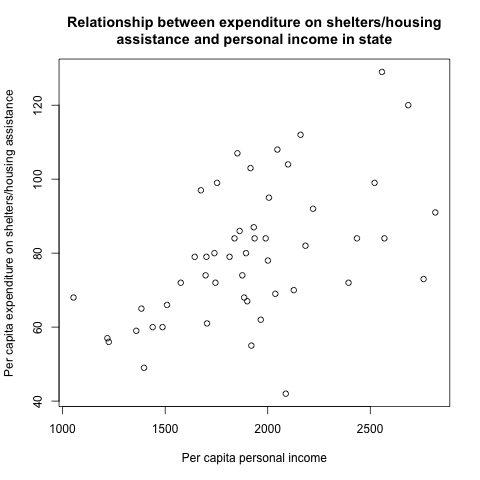
\includegraphics[width=0.5\textwidth]{scatterplot_y_x1.png}
\end{figure}

\noindent Figure 2 demonstrates a U-shaped distribution of the relationship between per capita state expenditure on shelters/housing and number of financially  insecure residents per 100.000 population. The visual analysis of the plot shows that below a certain margin (around 300 financially insecure residents per 100.000) the state expenditure decreases with an increase in the number of finacially insecure residents, however, above the margin, with higher numbers of financially insecure residents in state, this association turns positive. 

\begin{figure}[h!]\centering
	\caption{\footnotesize Expenditure and number of financially insecure residents}
	\label{fig:plot_2}
	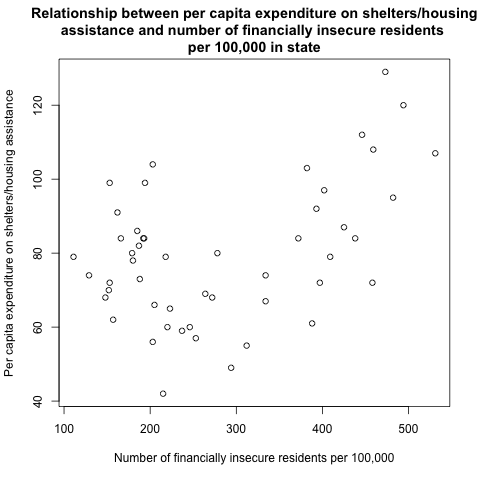
\includegraphics[width=.5\textwidth]{scatterplot_y_x2.png}
\end{figure}

\vspace{.2cm}
\noindent Figure 3 below shows a weak positive association between state expenditure on shelters/housing and the share of urban population: state expenditure increases with increasing number of urban residents. \\

\begin{figure}[h!]\centering
	\caption{\footnotesize Expenditure and number of people residing in urban areas}
	\label{fig:plot_3}
	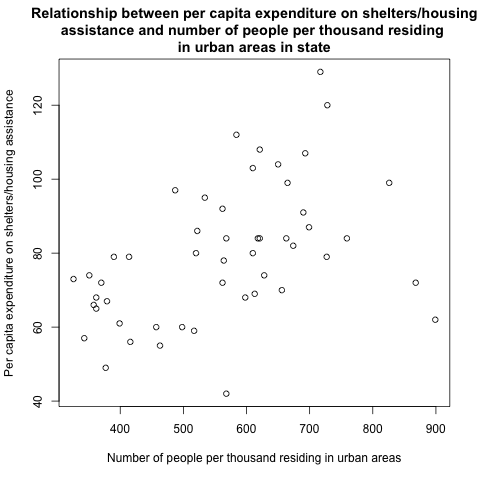
\includegraphics[width=.5\textwidth]{scatterplot_y_x3.png}
\end{figure}

\noindent Figure 4 shows the relationship between personal income and the number of financially insecure people in state. The visual investigation shows no association between these two variables. \\

\begin{figure}[h!]\centering
	\caption{\footnotesize Personal income and number of financially insecure residents}
	\label{fig:plot_4}
	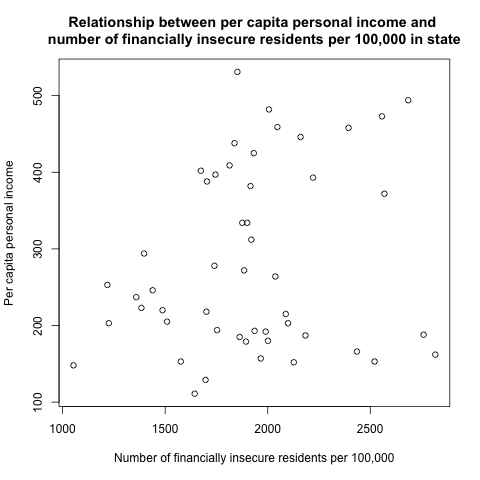
\includegraphics[width=.5\textwidth]{scatterplot_x1_x2.png}
\end{figure}

\noindent Figure 5 below shows a relatively strong positive association between per capita personal income and the number of people per thousand residing in urban areas, meaning with an increase in the number of urban residents in state there is an increase in the personal income. The data contains one extreme outlier which should be explored.  \\
\pagebreak

\begin{figure}[h!]\centering
	\caption{\footnotesize Personal income and number of people residing in urban areas}
	\label{fig:plot_5}
	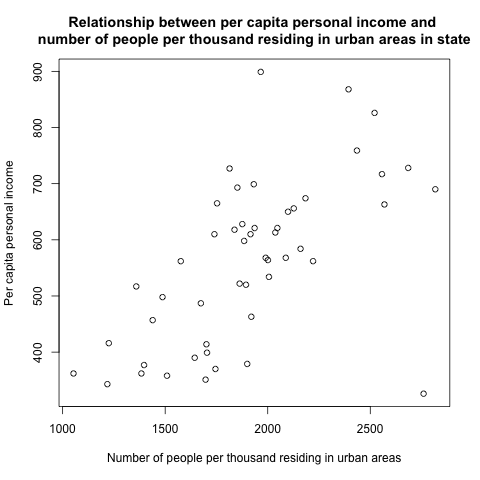
\includegraphics[width=.5\textwidth]{scatterplot_x1_x3.png}
\end{figure}

\noindent Figure 6 below shows a weak U-shaped distribution of the relationship between number of financially insecure residents and urban population in state or no association at all. The visual analysis of the plot shows that below a certain margin (around 300 urban residents) there is no association between the variables, however, above the margin there is a posible weak positive relationship.\\
\pagebreak

\begin{figure}[h!]\centering
	\caption{\footnotesize Number of financially insecure residents and number of people residing in urban areas}
	\label{fig:plot_6}
	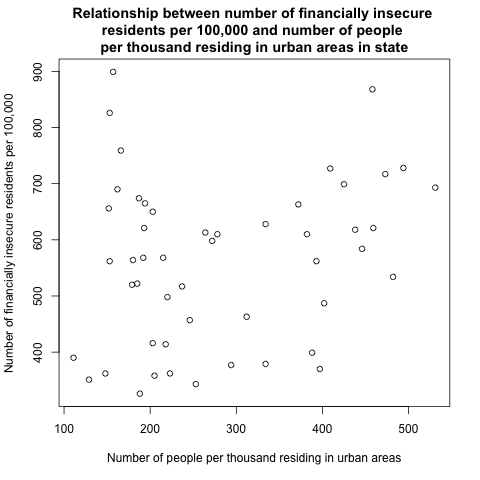
\includegraphics[width=.5\textwidth]{scatterplot_x2_x3.png}
\end{figure}

\noindent Next, we investigate the difference in state expenditure on shelters/housing assistance across regions. \\

\lstinputlisting[language=R, firstline=108, lastline=119]{PS01_answers_EK.R} 
\vspace{.2cm}

\noindent Figure 7 below shows the distribution of per capita expenditure shelters/housing assistance in state across the four regions. The states located in the "West" region have the highest per capita spending on shelters/housing assistance (88.31), while those located in the "Southeast" have the lowest (69.19). 
\pagebreak

\begin{figure}[h!]\centering
	\caption{\footnotesize Expenditure on shelters/housing assistance by region}
	\label{fig:plot_7}
	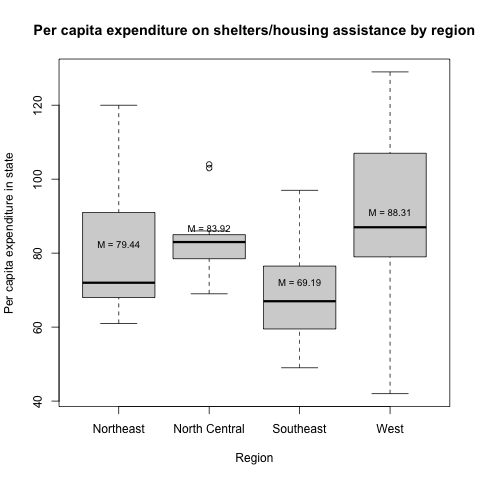
\includegraphics[width=0.7\textwidth]{boxplot_y_r.png}
\end{figure}

\noindent Lastly,we explore the relationship between expenditure on shelters/housing assistance and personal income across the four regions.\\

\lstinputlisting[language=R, firstline=121, lastline=134]{PS01_answers_EK.R} 
\pagebreak

\noindent Figure 8 below suggests there may be a difference in the strenth of the relationship between expenditure on shelters/housing assistance and personal income across the regions. Although the general relationship across all states looks positive, in case of "Southwest" it is strong positive, but is weak or none in case of other regions. 

\begin{figure}[h!]\centering
	\caption{\footnotesize Relationship between expenditure on shelters/housing assistance and personal income in state}
	\label{fig:plot_8}
	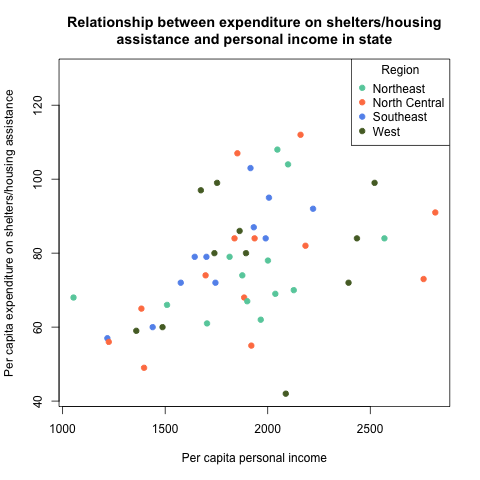
\includegraphics[width=0.7\textwidth]{scatterplot_y_x1_r.png}
\end{figure}

\end{document}
